%!TEX root = ../../adrien_gomar_phd.tex

Originally developed by \citet{He1998} and \citet{Ning1998},
the NLH method
relies on a decomposition of the conservative variables into a
time-averaged part plus an unsteady perturbation:
\begin{equation}
	u = \overline{u} + u^\prime,
	\label{eq:sm_nlh_decomposition}
\end{equation}
where $\overline{\vphantom{u}.}$ denotes the time-averaging operator and
$.^\prime$ its unsteady perturbation counterpart.
By injecting Eq.~\eqref{eq:sm_nlh_decomposition} into
Eq.~\eqref{eq:sm_nonlinear_convection_conservative}, one gets:
\begin{equation}
	\frac{\partial u^\prime}{\partial t} + 
	\frac{1}{2}\frac{\partial}{\partial x} \left[
	\overline{u}^2 + 2 \overline{u} u^\prime + u^\prime u^\prime \right] = 
	0.
	\label{eq:sm_nlh_step_1}
\end{equation}
The time-averaged equation can be obtained by time-averaging
equation~\ref{eq:sm_nlh_step_1}:
\begin{equation}
	(\overline{\ref{eq:sm_nlh_step_1}})
	\Leftrightarrow
	\frac{\partial}{\partial x}
	\left[\overline{u}^2 + 
	\overline{u^\prime u^\prime}\right] =
	0,
	\label{eq:sm_nlh_step_2}
\end{equation}
The term $\overline{u^\prime u^\prime}$
accounts for the non-linearities of the considered equation. It
is called the non-linear 
(or the deterministic) stress terms as a reference to 
the Reynolds stress terms. 
The equation for the unsteady perturbation is then obtained by keeping
the first order terms of the unsteady equation~\ref{eq:sm_nlh_step_1}.
This means that the term $u^\prime u^\prime$ is neglected and leads
to:
\begin{equation}
	\frac{\partial u^\prime}{\partial t} + 
	\frac{\partial}{\partial x} \left[\overline{u} u^\prime \right] = 
	0.
\end{equation}
Note that neglecting the high order terms 
(namely $u^\prime u^\prime$ for the Burger's equation) 
is almost similar to
linearizing the equation. However, in the NLH approach,
the time-averaged $\overline{u^\prime u^\prime}$ 
of $u^\prime u^\prime$ is kept in the
equation which takes into account for a part of the
non-linearities. Thus, the method is not linear.

\subsection{Mono-frequential formulation}
For now on, no assumption has been made neither on the velocity $u$,
nor on its time-averaged part and unsteady perturbation part.
Assuming that the velocity perturbation 
is periodic in time with period
$T=2 \pi / \omega$,
the unsteady perturbation can be decomposed into 
a Fourier series:
\begin{equation}
	u^\prime = \sum_{k=-\infty \atop k \neq 0}^{\infty} 
	\widehat{u}_k e^{i \omega k t}.
	\label{eq:sm_nlh_decomposition_pert}
\end{equation}
Since the complex exponentials family forms 
an orthogonal basis, we have for all harmonics 
$-\infty \leq k \leq \infty, \; k \neq 0$:
\begin{equation}
	i \omega k \widehat{u}_k + 
	\frac{\partial}{\partial x} \left[ \overline{u} \widehat{u}_k\right] =
	0.
	\label{eq:sm_nlh_decomposition_pert_part1}
\end{equation}
One can notice that the time-averaged part has been removed from
the Fourier series through $k \neq 0$ as it is computed 
separately in Eq.~\eqref{eq:sm_nlh_step_2}.
Each harmonic equation.~\eqref{eq:sm_nlh_decomposition_pert_part1}
represents now a steady equation as no temporal
derivative is present anymore.

The term $\overline{u^\prime u^\prime}$ remains in the time-averaged
equation and needs to be computed. It can be 
directly worked out when the harmonics are known:
\begin{equation}
	\begin{split}
		u^\prime u^\prime &= 
		\left[
			\sum_{k=-\infty \atop k \neq 0}^{\infty} \widehat{u}_k e^{i \omega k t} 
		\right]
		\left[
			\sum_{k=-\infty \atop k \neq 0}^{\infty} \widehat{u}_k e^{i \omega k t} 
		\right] \\
		&= \sum_{k=-\infty \atop k \neq 0}^{\infty} (\widehat{u}_k)^2
		   e^{i 2 \omega k t} +
		   2 \sum_{k,j=-\infty \atop k \neq j \neq 0}^{\infty} 
		   \widehat{u}_k \widehat{u}_j e^{i \omega (k + j) t}.
	\end{split}
\end{equation}
Thus,
\begin{equation}
	\begin{split}
		\overline{u^\prime u^\prime} &= 
		\frac{1}{T} \int_{t=0}^{T} \left[ 
			\sum_{k=-\infty \atop k \neq 0}^{\infty} (\widehat{u}_k)^2
		   	e^{i 2 \omega k t} +
		   	2 \sum_{k,j=-\infty \atop k \neq j \neq 0}^{\infty} 
		   	\widehat{u}_k \widehat{u}_j e^{i \omega (k + j) t} 
		\right] dt\\
		&= \frac{2}{T} \int_{t=0}^{T} \sum_{k,j=-\infty \atop k \neq j \neq 0}^{\infty} 
		   	\widehat{u}_k \widehat{u}_j 
		   	e^{i \omega (k + j) t} dt \\
		&= \frac{2}{T} \int_{t=0}^{T} 
			\sum_{k=-\infty \atop k \neq 0}^{\infty} 
			\widehat{u}_k \widehat{u}_{-k}  dt.
	\end{split}
\end{equation}
As $\widehat{u}_k$ and $\widehat{u}_{-k}$ are complex conjugates,
finally $\overline{u^\prime u^\prime}$ is equal to:
\begin{equation}
	\overline{u^\prime u^\prime} = 
	2 \sum_{k=-\infty \atop k \neq 0}^{\infty} |\widehat{u}_k|^2.
	\label{eq:sm_nlh_deterministic_stress_terms}
\end{equation}
This last equation depends only on the computed harmonics, meaning
that no term is modeled. Moreover, this term couples the
time-average solution with the unsteady perturbation. This precise
term is neglected in the linearized method seen in 
Sec.~\ref{sub:sm_lur}. It takes into account for the 
non-linearities of the considered equation.

Finally, as computing an infinite number of harmonics is 
numerically not feasible,
it is truncated at order $N$. 
This is a fair assumption as most
of the physical flows have a finite unsteady spectrum.
However, the goal of Fourier-based
methods is to have a compact representation of the unsteady time
signals. As for a mesh grid convergence, the number of harmonics $N$
is increased until the unsteady representation of the signal is
converged for the variable of interest. The discussion on the
convergence of Fourier-based methods will be detailed later on in this 
thesis \mytodo{ref chapitre}.

To summarize, the NLH
method applied to Eq.~\eqref{eq:sm_nonlinear_convection_conservative},
gives $2N$ perturbation equations and one time
averaged equation making $2N+1$ equations in total. 
A pseudo-time ($\tau$) derivative is
added to march the equations in pseudo-time to the steady-state 
solution of all the harmonics:
\begin{equation}
	\fbox{$
	\begin{dcases}
		\frac{\partial \overline{u}}{\partial \tau} + 
		\frac{\partial}{\partial x}
			\left[\overline{u}^2 + 
			\overline{u^\prime u^\prime}\right] &=
			0, \\
		\frac{\partial \widehat{u}_k}{\partial \tau} + 
		i \omega k \widehat{u}_k + 
			\frac{\partial}{\partial x} 
			\left[ \overline{u} \widehat{u}_k\right] &= 
			0, \: k \in [-N, N], \: k \neq 0.
	\end{dcases}
	$}
	\label{eq:sm_nlh_subset_eq}
\end{equation}
The equations are coupled by the deterministic 
stress term $\overline{u^\prime u^\prime}$
defined in Eq.~\eqref{eq:sm_nlh_deterministic_stress_terms}.
The term $u^\prime u^\prime$ is neglected in this formulation.

\subsection{Multi-frequential formulation}

\citet{He2002} extended the method to a multi-frequential
formulation. Instead of writing the perturbation
using a Fourier series as defined in Eq.~\eqref{eq:sm_nlh_decomposition_pert},
it is written using a sum of harmonics each of which
having an angular frequency $\omega_k$:
\begin{equation}
	u^\prime = \sum_{k=-N \atop k \neq 0}^{N} 
	\widehat{u}_k e^{i \omega_k t}.
	\label{eq:sm_nlh_decomposition_pert_multi}
\end{equation}
Note that the term $k \omega$ in Eq.~\eqref{eq:sm_nlh_decomposition_pert}
is now $\omega_k$ meaning that the frequencies can be chosen
arbitrarily.
The derivation of the equations is kept the same and the following
$2N+1$ subset of equations is finally obtained:
\begin{equation}
	\fbox{$
	\begin{dcases}
		\frac{\partial \overline{u}}{\partial \tau} +
		\frac{\partial}{\partial x}
			\left[\overline{u}^2 + 
			\overline{u^\prime u^\prime}\right] &=
			0, \\
		\frac{\partial \widehat{u}_k}{\partial \tau} + 
		i \omega_k \widehat{u}_k + 
			\frac{\partial}{\partial x} 
			\left[ \overline{u} \widehat{u}_k\right] &= 
			0, \: k \in [-N, N], \: k \neq 0.
	\end{dcases}
	$}
	\label{eq:sm_nlh_subset_eq_multi}
\end{equation}
However, as the complex exponentials do not form
an orthogonal basis, writing Eq.~\eqref{eq:sm_nlh_subset_eq_multi}
for each harmonic $k \in [-N, N], \: k \neq 0$ is mathematically
not true. \citet{He2002} argued that the terms
are collected for each harmonic. 
The same development is made by \citet{Vilmin2006}.

The coupling deterministic stress term is evaluated using the
same equation as for the mono-frequential formulation.
However, in the multi-frequential formulation, 
the equation Eq.~\eqref{eq:sm_nlh_deterministic_stress_terms}
is generally not true.
In fact, in the mono-frequential formulation, the term
\begin{equation}
	\frac{1}{T} \int_{t=0}^{T} (\widehat{u}_k)^2
		e^{i 2 \omega k t} dt.
	\label{eq:sm_nlh_int_deterministic}
\end{equation}
vanishes for each $k$ as the integral of the
exponential $e^{i 2 \omega k t}$ with respect to $t$
is given by $e^{i 2 \omega k t} / i 2 \omega k$ that is
periodic with period $T$. This means that the integral in 
Eq.~\eqref{eq:sm_nlh_int_deterministic} is equal to zero
for the mono-frequential formulation. 
However, in the multi-frequential
formulation, for some choice of frequencies, the period of all
of these may be difficult or even impossible to define. It
seems that mathematical justifications should be given
to be able to evaluate the deterministic stress term 
in the multi-frequential formulation
using Eq.~\eqref{eq:sm_nlh_deterministic_stress_terms}.

\subsection{Extensions}

\paragraph{Navier-Stokes equations}
As shown above, as the development of the NLH
method is made in the frequency domain, applying the method to
complex equations can be difficult. For the Navier-Stokes equations,
this step is tedious due to the number of equation to treat. Nevertheless, 
\citet{He1998, Chen2001, He2002, Vilmin2006} have
done this and the reader is referred to these papers
for a detailed description.
Note that in both publications, the turbulence is modeled
using only the time-averaged quantities.
This is another assumption as the turbulent field in a wake,
for instance, is seen unsteady in the opposite row frame
of reference~\cite{Lakshminarayana1980}. Thus, this
unsteadiness is not taken into account.

\paragraph{Turbomachinery computations}
Originally, the NLH method has been developed for 
turbomachinery applications. \citet{He1998} and
\citet{Ning1998} computed isolated turbomachinery
configurations. To reduce the domain to a single 
blade-to-blade passage, they consider a periodic
boundary condition for the time-averaged part and a
phase-lagged boundary condition for the perturbation on the
azimuthal boundaries:
\begin{equation}
    \begin{split}
    	\overline{u}_U &= \overline{u}_L, \\
    	u^\prime_U &= u^\prime_L e^{i \beta},
    \end{split}
\end{equation}
where subscript $U$ and $L$ denotes, respectively, 
the upper and the lower boundaries. $\beta$ is the
interblade phase angle. This allows to compute
isolated vibrating configurations thanks to 
\citet{Lane1956} theorem.
\citet{Chen2001} added a rotor-stator treatment
to allow for stage configurations. 
To do so, at the interface, the perturbation 
$u^\prime$ is exchanged using
an azimuthal Fourier transform. In opposite,
the time-average field $\overline{u}$ 
and the deterministic stresses 
$\overline{u^\prime u^\prime}$
are flux-averaged like in a mixing-plane approach.
Still the method is mono-frequential as only
one stage is considered, each row seeing the
opposite blade passing frequency. Considering
the time-averaged field to be constant in the azimuthal 
direction at the interface seems fair, but there is
no reason for $\overline{u^\prime u^\prime}$ to be.
\citet{He2002} extended the method to take into
account multi-stage configurations through the
development of a multi-frequential formulation.
In fact, in such an application, 
a sandwiched row will see unsteadinesses coming
from the upstream row (mainly wake effects) and
potential effects from the downstream rows. In the
general case where the surrounding rows do not have the
same blade passing frequencies, multiple frequencies
will be present in the current row. 
In this way, \citet{He2002} extended the NLH approach to
multi-frequential perturbation to allow such computations.
The same treatment is used at the rows interfaces meaning
that the time-averaged quantities are flux-averaged and the
fluctuations are exchanged through their azimuthal
Fourier transform.
\citet{Vilmin2006} extended the rotor-stator
interface to a non-matching join sliding mesh interface which
leads to the continuity of the unsteady flow field at the interface.
The main difference with the previous treatment is that
$\overline{u}$ and $\overline{u^\prime u^\prime}$ 
are not flux-averaged but rather spatially Fourier transformed,
which leads to the continuity of $u$ at the interface, when
the number of harmonics is sufficient.

\paragraph{Clocking effect}
\citet{He2002} extended the NLH method to
the computation of all clocking positions in one computation.
\begin{figure}[htbp]
  \centering 
  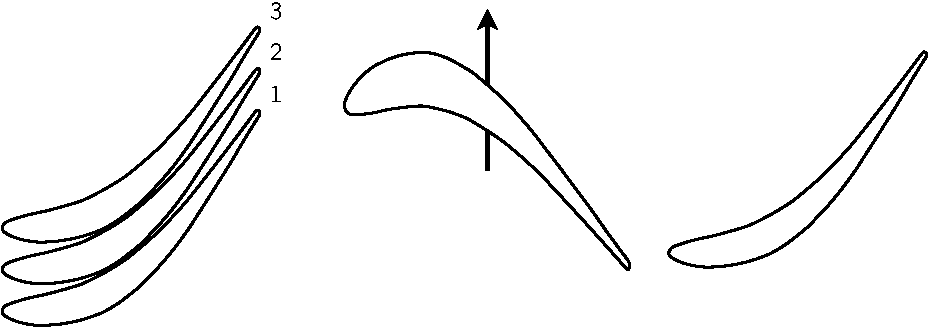
\includegraphics[width=.5\textwidth]{clocking_effect.pdf}
  \caption{Different clocking positions for a stator/rotor/stator
  configuration.}
  \label{fig:sm_nlh_clocking_effect}
\end{figure}
Fig.~\ref{fig:sm_nlh_clocking_effect} shows three
different clocking positions (sometimes also referred 
to as the indexing positions)
of the first stator
in a stator/rotor/stator configuration.
The relative position of both stator is of
prior interest. In fact, the wake that is shed behind the first stator
is cut by the rotor blades and transmitted to 
the second stator row. The stators being fixed, the wake of
the first stator is seen as a stationary wave in the second stator.
Hence, the importance of their relative position. For instance,
\citet{Huber1996} showed that
on their 1.5 turbine stage, the variation of efficiency due to clocking
position was equal to $0.8\%$ of efficiency, showing the
importance of the clocking effect.

The brute force to compute the clocking effect on a
configuration is to consider all relative positions. This means
that the geometry of the stator should be rotated for each new 
clocking position and hence a new unsteady computation should be 
run. The innovative procedure proposed by 
\citet{He2002} is to consider the clocking effect as a steady wave.
In fact, as both stator are fixed, a steady perturbation
generated behind the first stator is still steady in the second stator.
In terms of frequencies, a steady perturbation
can be assimilated to a zero frequency mode. 
In \citet{He2002} and \citet{Vilmin2009}, 
a perturbation with a zero frequency
is thus additionally computed. The clocking effect can then be evaluated by
post-processing the Fourier coefficient of the zeroth frequency mode.
Recently, the computation of clocking effects on
arbitrary configurations has been made possible
by \citet{Vilmin2013a}. This allows its use for 
pylon-rotor-rotor applications for instance, which
is the configuration encountered for an installed CROR.

\subsection{Cost of the method}
Compared to the LUR method, the number of equations to solve is 
not constant here. In fact, if $N$ denotes the number of harmonics
computed in total (sum of each harmonic of each perturbation)
and if $\mathdollar_{\text{RANS}}$ 
denotes the CPU and memory cost of
one steady computation, $2N$ harmonic equations and 
one time-average equation
are solved, thus:
\begin{equation}
	\mathdollar_{\text{NLH}} = (2N+1) \cdot \mathdollar_{\text{RANS}}.
\end{equation}
However, \citet{Vilmin2006} do not apply the NLH formulation
to the turbulent equation (in their case, 
the one equation of \citet{Spalart1992}),
since five equations are solved using the NLH approach and turbulent equation
is solved as a steady one,
the cost becomes:
\begin{equation}
	\mathdollar_{\text{NLH}} = \frac{5 \cdot (2N+1) + 1}{6} \cdot \mathdollar_{\text{RANS}}.
\end{equation}

